
\documentclass[11pt,a4paper,hidelinks,fleqn]{article}            % Article 12pt font for a4 paper while hiding links
\usepackage[margin=1in]{geometry}                          % Required to adjust margins
../styleAndCommands.tex
\date{}
\begin{document}

\subsection*{Question 1 [20 marks]}

\paragraph{a)} For the function $f(x) = x^4 + 2 x^2 - 5x, ~x\in[0, 10]$,
describe an algorithm for finding the root of $f'(x) = 0$ using the secant method.

Solution:
\begin{align*}
g(x) & = f'(x) = 4x^3 + 4 x - 5 \\
x_0 & = 0 \\
x_1 & = 10 \\
x_{i+1} & = x_i - g(x_i) [x_i - x_{i-1}] / [g(x_i) - g(x_{i-1})]
\end{align*}
until $x_{i+1} - x_{i} < \text{tolerance}$.

\paragraph{b)} Calculate the first two iterations of the secant method used in a).

Solution:
\begin{align*}
g(x_0) & = -5, ~g(x_1) = 4035, \\
x_2 & = 10 - 4035 \times 10 / 4040 = 0.0124, g(x_2) = -4.95, \\
x_3 & = 0.0124 + 4.95 \times (-9.9876) / (-4.95 - 4035) = 0.0224
\end{align*}


\subsection*{Question 2 [20 marks]} 

The function $f(x)$ is four times continuously differentiable ($C^4$).
Given 5 sample points of the function $[f(x_0-h), f(x_0-\frac{h}{2}), f(x_0), f(x_0+\frac{h}{2}), f(x_0+h)]$,
describe the algorithm to approximate $f'(x_0)$ through:

\vspace{-6mm}
\paragraph{a)} Taylor expansion at the four points $f(x_0-h), f(x_0-\frac{h}{2}), f(x_0+\frac{h}{2}), f(x_0+h)$;

Solution:
The Taylor expansion multiplied by $b_i$ is
\begin{align*}
\begin{cases}
b_1 f(x - h) & = b_1 [f(x) - f'(x)h + \frac12 f''(x)h^2 - \frac16 f^{(3)}(x)h^3] \\
b_2 f(x - \frac12 h) & = b_2 [f(x) - f'(x) \frac12 h + \frac12 f''(x) \frac14 h^2 - \frac16 f^{(3)}(x)\frac18 h^3] \\
b_3 f(x + \frac12 h) & = b_3 [f(x) + f'(x) \frac12 h + \frac12 f''(x) \frac14 h^2 + \frac16 f^{(3)}(x) \frac18 h^3] \\
b_4 f(x + h) & = b_4 [f(x) + f'(x)h + \frac12 f''(x)h^2 + \frac16 f^{(3)}(x)h^3]
\end{cases}
\end{align*}
We would like the sum of the right hand sides to be equal to $f'(x)$, 
so the $b_i$'s have to satisfy the linear system:
\begin{align*}
\begin{cases}
& -b_1 - \frac12 b_2   + \frac12 b_3 + b_4 = \frac1h \\
& b_1  + \frac14 b_2  + \frac14 b_3 + b_4 = 0   \\
& b_1  + b_2      + b_3     + b_4 = 0   \\
& -b_1 - \frac18 b_2  + \frac18 b_3 + b_4 = 0   
\end{cases} 
\Rightarrow  \vec{M} \vec{b} = \left[\frac1h\ 0\ 0\ 0 \right]^{\top}
\Rightarrow  \vec{b} = \vec{M}^{-1}\left[\frac1h\ 0\ 0\ 0 \right]^{\top}
\end{align*}
And sum of the left hand side is $\sum_i cs_i y_i = f'(x)$, where $cs = [b_1, b_2, 0, b_3, b_4] $.


\paragraph{b)} Richardson extrapolation with the central difference g(h) and the step sizes $h$ and $\displaystyle \frac{h}{2}$; 

Solution:

The central differences are
\begin{align*}
& g(h) = \frac{f(x+h) - f(x-h)}{2h} \\
& g\left(\frac{h}{2}\right) = \frac{f(x+\frac h 2) - f(x-\frac h 2)}{h}
\end{align*}
Richardson extrapolation:
\begin{align*}
f'(x) = \frac43 g\left(\frac{h}{2}\right) - \frac13 g(h) = \frac1{6h} f(x-h) - \frac{4}{3h} f(x-\frac{h}2) + \frac{4}{3h} f(x+\frac{h}2) - \frac1{6h} f(x+h)
\end{align*}


\paragraph{c)} constructing the polynomial of order 4, $p(x) = \sum_{i=0}^4 a_i x^i$, passing the 5 given points and taking the derivative of the polynomial at $x_0$.

Solution:

Given five points we can fit a 4th order polynomial 
\begin{align*}
y = a_4 x^4 + a_3 x^3 + a_2 x^2 + a_1 x + a_0
\end{align*}
by solving the linear system $\vec{M} \vec{a} = \vec{y}$, where
\begin{verbatim}
M  = [(x0-h)^4, (x0-h)^3, (x0-h)^2, (x0-h), 1;
      (x0-h/2)^4, (x0-h/2)^3, (x0-h/2)^2, (x0-h/2), 1;
      x0^4, 	x0^3, 	  x0^2,     x0,     1;
      (x0+h/2)^4, (x0+h/2)^3, (x0+h/2)^2, (x0+h/2), 1;
      (x0+h)^4, (x0+h)^3, (x0+h)^2, (x0+h), 1;]
\end{verbatim}
So the coefficients of the polynomial $\vec{a} = \vec{M}^{-1} \vec{y}$.
And 
\begin{align*}
f'(x) = [4x^3, 3x^2, 2x, 1, 0]^\top \vec{a}
\end{align*}



\subsection*{Question 3 [20 marks]}
Consider the following one step binomial tree model of the stock price process:
\begin{figure*}[h]
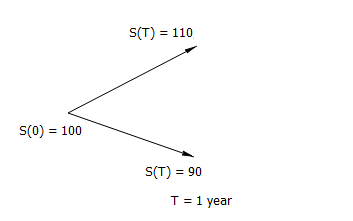
\includegraphics[scale=0.9]{./4}
\end{figure*}

a) Assume interest rate is $0\%$, compute the price of a call option struck at 100 at maturity 1 year?

Solution: risk neutral probability: 50\%, 50\%. option price $= 10 \times 0.5 + 0 * 0.5 = 5$.

b) Assume interest rate is $5\%$, compute the price of a call option struck at 100 at maturity 1 year?

Solution: risk neutral probability: 75\%, 25\%. option price $= 10 \times 0.75 + 0 * 0.5 = 7.5$.


\subsection*{Question 4 [20 marks]} 
Consider the numerical integration of 
\begin{align*}
\int_0^{10} \frac{1}{2} e^{-\frac12x^2} dx
\end{align*}

\paragraph{a)} Evaluate the integral by mid-point quadrature with 4 equally spaced intervals. 

\paragraph{b)} Describe in pseudo code the algorithm to evaluate the integral using Monte-Carlo simulation.
 
\paragraph{c)} What change do you need to make in the Monte-Carlo integration in b)
if you would like to use the first 2 terms of the Taylor series
expansion of $e^{-\frac12 x^2}$ as control variate?


\subsection*{Question 5 [20 marks]}
Consider the process of a underlying asset's price $X_t$
\begin{align*}
dX_t = \sigma dW_t
\end{align*}
where $W_t$ is a standard Wiener process and $\sigma$ is the constant volatility.
Denote $V_t$ the price of a derivative on the asset. 

a) Derive the partial differential equation satisfied by $V(x, t)$.

b) Discretize the partial differential equation using explicit Euler scheme in time axis and central different in price axis,
write down the equation that computes $V(x, t_i)$ from the time slice $t_{i+1}$.

c) Suppose that the derivative's price at $t_{i+1}$ is of the form shown in the below chart,
i.e., $V(x, t_{i+1})$ is known, 
sketch the rough shape of $V(x, t_{i})$ on top of the plot and explain the rationale.
\begin{figure*}[h]
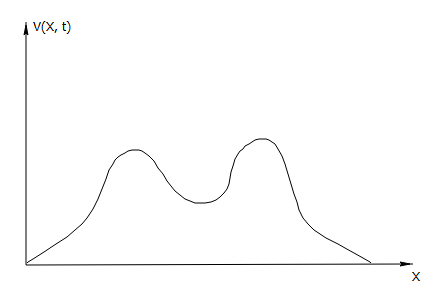
\includegraphics[scale=0.9]{./6c} \\
\vspace{1cm}
\textbf{*END OF PAPER*}
\end{figure*}



\end{document}
